\chapter{USR@istar: ultrafast shape recognition}
\label{usr}

\section{Abstract}

Finding compounds structurally similar to a query ligand has been an important but daunting problem for a long time. The USR (Ultrafast Shape Recognition) algorithm represents a whole new alignment-free method that encodes the shape information semantically and permits superfast screening of a large molecular database. A few extensions to USR improve the original method from various perspectives and three of some, UFSRAT, EDULISS and SwissTargetPrediction, are also available as web servers. However, UFSRAT and EDULISS are unable to discriminate between long, chain-like molecules, and their calculated distributions are not meaningful when some pharmacophoric features are rarer than others. SwissTargetPrediction uses a small, well annotated, bioactive compound database and is generally for target fishing.

For prospective virtual screening purposes, in this study we implementated USR and its USRCAT (USR with Credo Atom Types) extension on top of our istar web platform. We re-used the large molecular database of more than 23 million diverse ligands that originally came with idock, and exploited three levels of parallelism with a novel implementation of sum of absolute different using AVX (Advanced Vector Extensions) to accelerate similarity score calculation. Our USR@istar supports a query ligand in either SDF, MOL2, XYZ, PDB or PDBQT format, and interfaces with our iview WebGL visualizer for interactive visualization of high-score hits. USR@istar is freely available at http://istar.cse.cuhk.edu.hk/usr.

This is an ongoing collaborative project with Pedro J. Ballester from Cancer Research Center of Marseille, Marseille, France.

\section{Background}

Molecular shape has been widely acknowledged as a key factor for biological activity and thus is regarded as a very important pattern for which to search. Searching the molecular database for compounds that most closely resemble the shape of a given query molecule, be it a known inhibitor of a target protein, a natural product, or even a patented compound, finds pragmatic applications in ligand-based virtual screening \citep{1332,1380,1281,1504,1502} and target fishing \citep{1528,1407,1408,1402}. Therefore molecular similarity search assists in discovering structurally novel active compounds, or in identifying potential interacting target of bioactive ligands, which is useful for understanding the polypharmacology and safety profile of existing drugs. Furthermore, this approach can be applied to other scientific disciplines such as performing similarity comparisons between proteins or designing content-based Internet search engines for 3D geometrical objects \citep{1280}.

The molecular shape similarity can be quantified by methods based on structural alignment \citep{1440,887,1439,1534} or shape recognition \citep{1379,1338,1331}. Structural alignment is also known as molecular superposition and requires precise geometric comparison which is often computationally demanding. Shape recognition, on the other hand, encodes shape information into a numerical feature vector, which can be subsequently used to compute a similarity score between two molecules very efficiently.

USR (Ultrafast Shape Recognition) \citep{1379} was the very first non-superposition method for molecular shape comparison, and demonstrated superior computational performance at least three orders of magnitude faster than previously existing alignment-based methods. USR has another major advantage of being invariant to spatial rotation and translation, and hence circumvents the problematic requirement of aligning molecules. USR defines the shape of a molecule independently and for every molecule uses a fixed set of 12 descriptors derived from the first 3 statistical moments of distributions of interatomic distances between atoms and 4 purposely-selected centroids. This encoding ensures that every molecule will have a unique location in the 12-dimensional chemical space spanned by the used descriptors, and consequently enables finding and visualizing clusters of molecules with similar shape \citep{1280,1332}. Selecting the most representative molecule of each cluster could be applied to avoid repeating expensive biological tests on similar molecules \citep{1280}. The ability of USR as a standalone method was studied to identify molecules sharing common biological activities through retrospective \citep{1332} and prospective \citep{1380,1281,1504,1502,1615} virtual screening experiments. Prospectively, USR was applied to the discovery of inhibitors of arylamine NATs (N-acetyltransferases) \citep{1380}, DHQase2 (dehydroquinase type 2) \citep{1281}, PAD4 (protein arginine deiminase type 4) \citep{1504}, p53-MDM2 (murine double minute 2) \citep{1502}, and PRL-3 \citep{1615}. USR was also used for deduplication in a virtual screening campaign \citep{1390} and in our iSyn \citep{1409,1387} \textit{de novo} ligand deisgn software.

Since USR was developed in 2007, there have been quite a few extensions \citep{1333,1436,1437,1334,1335,1337,1338,1331,1407,1408} to augment the original method. \citep{1333} presented a hybrid approach composed of USR and the topological MACCS key descriptors, which are binary in nature and encode the presence or absence of 166 predefined structural fragments. It used the first four unbalanced moments of each distribution of atomic distances and incorporated additional chemical information through 2D structural similarity. Random Forest \citep{1309} was used for multi-class classification. Incorporating an additional central moment, the kurtosis, was found to significantly improved its performance. The addition of the fifth central moment, however, did not improve the performance sufficiently to justify the increased computational expense.

UFSRAT \citep{1436} addressed the lack of discrimination between compounds having similar shape but distinct pharmacophoric features by subdividing atoms into four subsets which are heavy, hydrophobic, hydrogen bond acceptor or donor atoms, according to their atom types. For each subset, the four centroids were calculated, and so were the 12 USR descriptors. Therefore 48 descriptors were resulted. This was to ensure that similar compounds are able to make the same type of interactions within biological systems as the query ligand. UFSRAT was prospectively applied to the discovery of inhibitors of 11$\beta$-HSD1 (hydroxysteroid dehydrogenase type 1) \citep{1505}. UFSRAT is available as a web server at http://opus.bch.ed.ac.uk/ufsrat/. There are 28 databases to search against, with the largest one containing 4,853,000 conformers. UFSRAT is also employed for geometrical similarity searches in the EDULISS database \citep{1437} available at http://eduliss.bch.ed.ac.uk/ which comprises over 5 million commercially available compounds.

CSR \citep{1334} and USR:OptIso \citep{1335} attempted to tackle the lack of discrimination between chiral compounds. Their novel idea was to position the centroids in such a way that they clearly distinguish between enantiomers, i.e. optical isomers. They both used cross product because it is an operator that transforms equivariantly under rotations and translations, but not under reflections. The two methods differed in selecting the centroids and in replacing or supplementing the new optical isomerism descriptor \citep{1335}. CSR \citep{1334} was tested on the DUD (Directory of Decoys) dataset \citep{87}, where a significant improvement in enrichment was found over USR. USR:OptIso \citep{1335} was shown to be helpful for analyzing molecules with stereogenic centers, atropisomerism, and in the clustering of conformers generated by systematic bond rotation.

ElectroShape \citep{1337,1338} extended the CSR \citep{1334} method by encoding electrostatics and liphophilicity through additional dimensions and centroids. In \citep{1337}, the partial charge was represented as a fourth coordinate, with atoms being identified by points in four-dimensional space. ElectroShape was validated using release 2 of the DUD dataset \citep{87}, and showed a near doubling in enrichment over USR and CSR. Different implementations of partial charge were also revealed to affect the enrichment performance significantly. The addition of a fourth statistical moment, as was done in \citep{1333}, improved USR and CSR but not ElectroShape, suggesting that adding extra information might not necessarily improve enrichment but could dilute the information already included. In \citep{1338}, ElectroShape was further extended by using atomic lipophilicity as an additional molecular property, with atoms being identified by points in five-dimensional space. This version of ElectroShape showed a clear improvement in performance, indicating that adding extra independent atomic properties makes shape-based enrichments even better.

USRCAT \citep{1331} extended the UFSRAT \citep{1436} method by identifying five subsets of atoms with the help of the SMARTS patterns used for atom typing in the CREDO database \citep{522,1530}. The five subsets were chosen to be heavy, hydrophobic, aromatic, hydrogen bond acceptor or donor atoms. Aromaticity was added to USRCAT as a pharmacophoric subset because USR was unable to discriminate between long, chain-like molecules such as certain heteropeptides and long alkylchains in particular. Unlike UFSRAT \citep{1436}, USRCAT \citep{1331} derived the four centroids from heavy atom coordinates and used them to calculate the distributions for all the five subset moments to improve screening performance. USRCAT was shown to outperform the traditional USR method in a retrospective virtual screening benchmark with the DUD-E (Directory of Decoys, Enhanced) dataset \citep{1185}. The highest enrichment factors were only achieved if the LEC (Lowest Energy Conformer) of an active was used as a query and if the LECs were included in the target set, but this observation cannot be generalized. DUD-E was found to be not ideal to benchmark the virtual screening performance of global shape similarity algorithms such as USR and its variants due to the large variations in molecular size of the active ligands.

A recent study \citep{1407} used a reference set of 224,412 molecules active on 1,700 human proteins and showed that accurate target prediction can be achieved by using a multiple logistic regression to combine different measures of chemical similarity based on both chemical structure and molecular shape, with the former using FP2 fingerprints and the latter using ElectroShape \citep{1338}. This hybrid method was later developed into the SwissTargetPrediction \citep{1408} web server, available at http://www.swisstargetprediction.ch/, to identify new targets for uncharacterized molecules or secondary targets for known molecules. With data collected from the ChEMBL database version 16 \citep{1441}, the molecular library was expanded to 280,000 compounds active on 2,686 targets of the organisms of human, mouse, rat, cow and horse. Mapping predictions by homology within and between different species, a powerful approach to translate results obtained in model organisms to human, were enabled for close paralogs and orthologs.
%\citep{1531} Atom Pair 2D-Fingerprints Perceive 3D-Molecular Shape and Pharmacophores for Very Fast Virtual Screening of ZINC and GDB-17. http://www.gdb.unibe.ch/

\section{Motivation}

Among the USR variants mentioned above, only three of them \citep{1436,1437,1408} have been made available as web servers together with different databases for different purposes. The UFSRAT \citep{1436} and EDULISS \citep{1437} web servers both employ the UFSRAT \citep{1436} method for ligand similarity search. However, as pointed out in \citep{1331}, this method is incapable of discriminating between long, chain-like molecules such as certain heteropeptides and long alkylchains because aromaticity is not considered as a pharmacophoric subset; besides, calculating the four centroids for each set of atoms individually is problematic because either the parameters cannot be calculated at all or the underlying distance distributions are not with respect to the overall shape of a molecule and not meaningful when some pharmacophoric features are rarer than others. The UFSRAT \citep{1436} web server constrains the input query ligand to be one molecule in SDF format only, and implements no online visualization. The EDULISS \citep{1437} web server requires drawing a query structure in a Java molecular editor, which is being disabled on more and more systems due to security concerns. The SwissTargetPrediction \citep{1408} web server, on the other hand, comprises well-annotated active compounds and is primarily used for predicting the target proteins of bioactive small molecules but not for prospective virtual screening purposes.

\section{Objective}

In this project we aimed to provide an istar-based \citep{1362} web service for large-scale prospective virtual screening using USR-like methods. We chose to employ USR \citep{1379} and USRCAT \citep{1331} because they have demonstrated pragmatic usefulness in prospective \citep{1380,1281,1504,1502} and retrospective \citep{1331} virtual screening experiments, respectively, and their source code is freely available for studying the precise implementation and porting to other programming languages such as C++ and JavaScript. Our USR@istar has several distinctive features. First, it uses both USR and USRCAT to search a large database comprising 23 million compounds collected from ZINC \citep{532,1178}. Second, it utilizes three levels of parallelism, both coarse grained and fine grained, to accelerate job execution. Third, it supports a query ligand in one job in five formats, and interfaces with the iview \citep{1366} WebGL visualizer to display results in an interactively manner.

\section{Methods}

This section first reviews the general methods of USR \citep{1379} and USRCAT \citep{1331}, and then introduces their specific implementations on our istar platform \citep{1362}.

\subsection{USR and USRCAT}

USR is based on the observation that the shape of a molecule is uniquely determined by the relative position of its atoms, which is in turn determined by the set of all interatomic distances. This convenient representation is independent of molecular orientation or position, and thus eliminates any need for alignment or translation. The interatomic distances are heavily constrained by the forces that hold the atoms together, and hence they contain more than sufficient information to accurately describe molecular shape. So it is possible to use a set of all atomic distances from a small number of strategic reference locations uniquely defined in every molecule and meanwhile retain the discriminative power necessary to distinguish between molecules.

The four reference locations are selected to be the molecular centroid (ctd), the closest atom to ctd (cst), the farthest atom to ctd (fct), and the farthest atom to fct (ftf). These locations represent the centre of the molecule and its extremes, and thus are well separated. In this way molecular shape is described by four distributions of atomic distances, where the number of atomic distances is proportional to the number of atoms. In order to compare molecules with different number of atoms, the first three moments of these distributions are computed and used to encode the shape information instead. These moments have semantics indeed. For instance, the 1st, 2nd and 3rd moments of distribution of atomic distances to the molecular centroid (ctd) capture the size, variance and skewness of the molecule, respectively. Selecting the first three moments provides an excellent compromise between the efficiency and the effectiveness of the method. Finally the shape similarity score of two molecules is calculated through the sum of absolute differences of their respective moments.

In this study the first three moments are computed in the same way as in ElectroShape \citep{1337}, which is slightly different than the way used in USR \citep{1379,1332,1380} and USRCAT \citep{1331}. Mathematically, for a distribution of atomic distances $\{d_k\}_{k=1}^n$ to one of the four reference locations (ctd, cst, fct, ftf), where $n$ is the number of atoms, the first three moments are semantically the mean, the standard deviation, and the cube root of the third central moment, respectively. Their exact expressions are shown in equations \eqref{usr:moment1}, \eqref{usr:moment2} and \eqref{usr:moment3}. The roots are intended to provide all moments with linear space dimension in \AA, unlike the skewness, for instance, which is unitless. This computation allows the distributions to contain only one sample, in which case the 2nd and 3rd moments will be zeros, i.e. $\mu_2=\mu_3=0$ when $n=1$. Likewise, when a distribution contains only two samples, the 3rd moment will be zero, i.e. $\mu_3=0$ when $n=2$.

\begin{equation}
\mu_1=\frac{1}{n}\sum_{k=1}^{n}{d_k}
\label{usr:moment1}
\end{equation}

\begin{equation}
\mu_2=\sqrt[2]{\frac{1}{n}\sum_{k=1}^{n}{(d_k-\mu_1)^2}}
\label{usr:moment2}
\end{equation}

\begin{equation}
\mu_3=\sqrt[3]{\frac{1}{n}\sum_{k=1}^{n}{(d_k-\mu_1)^3}}
\label{usr:moment3}
\end{equation}

After a molecule is encoded into a 12-element numerical moment vector $\mathbf M=(\mu_1^{ctd}, \mu_2^{ctd}, \mu_3^{ctd}, \mu_1^{cst}, \mu_2^{cst}, \mu_3^{cst}, \mu_1^{fct}, \mu_2^{fct}, \mu_3^{fct}, \mu_1^{ftf}, \mu_2^{ftf}, \mu_3^{ftf})$, the dissimilarity score of two molecules $\mathbf M^i$ and $\mathbf M^j$ can be defined as the sum of absolute differences of their respective moments, much like the city block distance. Thereafter, this dissimilarity is monotonically inverted so as to transform it into a normalized similarity score using equation \eqref{usr:usrscore}, where the minimum shape similarity is represented by score 0 and the maximum similarity by score 1. Any other inverse monotonic function can do this transformation if it preserves the ranking order.

\begin{equation}
S(\mathbf M^i, \mathbf M^j)=(1+\frac{1}{12}\sum_{k=1}^{12}|\mathbf M_k^i-\mathbf M_k^j|)^{-1}\in[0, 1]
\label{usr:usrscore}
\end{equation}

USR \citep{1379} is highly extensible via positioning reference locations \citep{1334,1335}, incorporating higher orders of moments \citep{1333,1337}, expanding coordinate dimensions \citep{1337,1338}, mixing chemical component similarity \citep{1333,1407,1408}, or subdividing atoms into subsets \citep{1436,1331}. USRCAT \citep{1331} extends USR \citep{1379} by separately identifying five pharmacophoric subsets of atoms, which are heavy, hydrophobic, aromatic, hydrogen bond acceptor or donor atoms. Consequently the resulting moment vector is expanded from 12 descriptors to 60, with the first 12 being identical to USR moments. In the case of an empty subset, for examples if no hydrogen bond donors are found, the corresponding elements in the moment vector are set to zero. The four reference locations are uniformly derived from heavy atom coordinates and are thus meaningful with respect to the overall shape of a molecule. The five sets of 12 moments are individually scaled by the factors $ow$ for all atoms, $hw$ for hydrophobic atoms, $rw$ for aromatic atoms, $aw$ for hydrogen bond acceptors and $dw$ for hydrogen bond donors, as shown in equation \eqref{usr:usrcatscore}. Without a prior knowledge, the values of the five scaling factors are all defaulted to one. USRCAT degenerates to USR when $ow=1$ and $hw=rw=aw=dw=0$.

\begin{eqnarray}
S(\mathbf M^i, \mathbf M^j)=(1
&+&ow\times\frac{1}{12}\sum_{k= 1}^{12}|\mathbf M_k^i-\mathbf M_k^j|\nonumber\\
&+&hw\times\frac{1}{12}\sum_{k=13}^{24}|\mathbf M_k^i-\mathbf M_k^j|\nonumber\\
&+&rw\times\frac{1}{12}\sum_{k=25}^{36}|\mathbf M_k^i-\mathbf M_k^j|\nonumber\\
&+&aw\times\frac{1}{12}\sum_{k=37}^{48}|\mathbf M_k^i-\mathbf M_k^j|\nonumber\\
&+&dw\times\frac{1}{12}\sum_{k=49}^{60}|\mathbf M_k^i-\mathbf M_k^j|)^{-1}\in[0, 1]
\label{usr:usrcatscore}
\end{eqnarray}

\subsection{USR and USRCAT on istar}

Like in idock@istar for prospective structure-based virtual screening, we used the same database, which comprises 23,129,083 ligands collected from the All Clean Subset of ZINC \citep{532,1178}.

It is helpful to include more than one conformer per compound in the database since flexible molecules can adopt different shapes. Hence the more of these conformations that are included in the database, the less likely it is to miss molecules with the desired pattern. Each small organic molecule could have an average of about 200 conformations \citep{1332}, or up to 292 conformations \citep{1280}. The conformers of a particular molecule are in general geometrically distinct and have low potential energy, as conformers with high internal energy are in principle less likely to occur in nature.

There are numerous 2D-to-3D conversion tools that can generate 3D molecular conformations from a considered 2D chemical structure, such as Cyndi \citep{1393,1394} and OMEGA \citep{462}. A study \citep{1127} examined the performance of four freely available small molecule conformer generation tools, Balloon \citep{1442}, Confab \citep{1443}, Frog2 \citep{1444}, and RDKit (http://www.rdkit.org/), alongside a commercial tool, MOE (http://www.chemcomp.com/), and found that RDKit and Confab were statistically better than other methods at generating low RMSD (Root Mean Square Deviation) conformers to the known structure, and RDKit resulted as the second fastest method after Frog2. The positive results for RDKit in terms of accuracy and speed make it a valid free alternative to commercial, closed source, proprietary software.

However, even though the conformers generated by RDKit can be ensured to be at least a certain RMSD threshold apart from each other by setting an appropriate parameter, they are not guaranteed to be of low energy, so it is suggested by the manual to energy minimize them using RDKit's implementation of the Universal Force Field (UFF). After energy minimization, unfortunately, some conformers could fall into the same local energy minimum and again become structurally similar to each other with RMSD below the threshold. To resolve this conformational diversity problem, the study \citep{1127} also described a postprocessing algorithm to discriminate and keep only conformers which are both energy minimized and a certain RMSD threshold apart. In the postprocessing algorithm, the energy minimized conformers are first sorted by increasing energy value and the lowest energy conformer is retained, and then for each of the remaining conformers, it will be discarded when its RMSD from any conformers that have been retained is smaller than a fixed threshold $d_{min}$, or it will be retained otherwise. The study \citep{1127} also suggested optimal values of the number of conformers to generate ($n_c$ in equation \eqref{usr:n_c}, where $n_{rot}$ is the number of rotatable bonds) and the $d_{min}$ value of 0.35\AA. Using RDKit in combination with the postprocessing algorithm, one can quickly build a diverse and representative set of conformers.

\begin{equation}
n_c=
\begin{cases}
 50 & \text{if } n_{rot} \leq 7\\
200 & \text{if } 8 \leq n_{rot} \leq 12\\
330 & \text{otherwise}\\
\end{cases}
\label{usr:n_c}
\end{equation}

Due to the superior accuracy and speed of RDKit, in this study we proposed to use RDKit together with the postprocessing algorithm to generate conformers. Precisely, we would use RDKit version 2014.09.1 and program against its C++ API instead of directly using the example Python script, and adopt the optimal parameter values suggested in \citep{1127}. Conformer generation is yet to be implemented in the near future.%TODO: add a histogram to show the number of conformers of each molecule, and mention the total and average number.

Suppose after generating approximately 10 conformers on average for each molecule, the database would contain 230 million conformers, each of which has a USRCAT moment vector of 60 elements of double precision floating point type, which requires 64 bits, or 8 bytes for storage. This sums up to $8B*60*230M=108GB$ for the size of the USRCAT descriptors of all conformers in the entire database.

On one hand, given a server with sufficient capacity of memory, it is possible to preload all descriptors to enable fast screening. Mathematically, suppose $t_{read}$ is the reading time of a moment vector of a conformer in the database, $t_{score}$ is the scoring time of two moment vectors, $n_{conf}$ is the number of conformers in the database, $n_{query}$ is the number of query ligands of a single job, and $n_{job}$ is the number of jobs, the total screening time $t$ would be

\begin{equation}
t=t_{read}\times n_{conf}+t_{score}\times n_{conf}\times n_{query}\times n_{job}
\label{usr:time0}
\end{equation}

On the other hand, on a server with insufficient memory to preload all descriptors, it is possible to load the descriptors chunk by chunk whenever a new job gets executed. Suppose only $m_{conf} << n_{conf}$ moment vectors fit in the memory. The chunk-by-chunk approach is to loop for $n_{conf}/m_{conf}$ times, each time loading a different chunk with $m_{conf}$ moment vectors and then making the $n_{query}$ queries on this chunk. In this way, the total screening time $t$ would be

\begin{eqnarray}
t&=&(t_{read}\times m_{conf}+t_{score}\times m_{conf}\times n_{query})\times(n_{conf}/m_{conf})\times n_{job}\nonumber\\
 &=&t_{read}\times n_{conf}\times n_{job}+t_{score}\times n_{conf}\times n_{query}\times n_{job}
\label{usr:time1}
\end{eqnarray}

As seen from the above screening time analysis, there are apparently several levels of parallelism to exploit. On the server side, there are millions of conformers, each of which has a moment vector of 60 elements. On the client side, there are multiple job submissions, each of which contains multiple queries. In the chunk-by-chunk approach, the scoring of the current chunk and the reading of the next chunk can even be pipelined.

Considering the fundamental architecture of our istar platform \citep{1362} as well as the nature of the problem, we decided to exploit three levels of parallelism: multiple jobs are broadcast to multiple daemons running on multiple servers; multiple queries are broadcast to multiple CPU cores of a server; multiple descriptors are broadcast to multiple vector registers of a CPU core. The first two levels of parallelism are coarse grained and easy to implement, whereas the third level is relatively fine grained and requires the support of, for instance, AVX (Advanced Vector Extensions).

AVX are extensions to the x86 instruction set and expand the width of the SIMD (Single Instruction, Multiple Data) register file to 256 bits. Such a 256-bit register can hold four USR or USRCAT descriptors of 64-bit double precision floating point type. In view of the fact that a USR or USRCAT moment vector can be expressed as $\mathbf M=(M_1, M_2, M_3, M_4, \ldots, M_n)$ for indexing purpose, where $n=12$ for USR and $n=60$ for USRCAT, this moment vector can be decomposed into groups of four elements, which are processed using AVX in a SIMD fashion as shown in Figure \ref{usr:AVX}. Specifically, to compute the USR or USRCAT scores between two moment vectors $\mathbf M^i$ and $\mathbf M^j$ in equation \eqref{usr:usrscore}, the sum of absolute differences of their respective moments must be first calculated. This can be done ideally using AVX in four steps: firstly, the four elements are subtracted; secondly, the most significant bits of the four elements are set to zeros; thirdly, the four elements undergo a horizontal addition; and lastly, the first and third elements are summed up. Note that the above four steps compute the sum of absolute differences of four respective moments only, so they are wrapped inside a loop where the number of iterations is 3 for USR and 15 for USRCAT so as to compute the sum of absolute differences of all respective moments. The calculations of USR and USRCAT scores can be merged in one loop because the first 3 iterations for USRCAT are literally also for USR (equation \eqref{usr:usrcatscore}). Since the loop count is constant and both the moment vectors are indexed constantly, unrolling is applicable here, resulting in a longer sequence of instructions but faster execution due to the circumvention of the use of a loop iterator.

\begin{figure}
\begin{center}
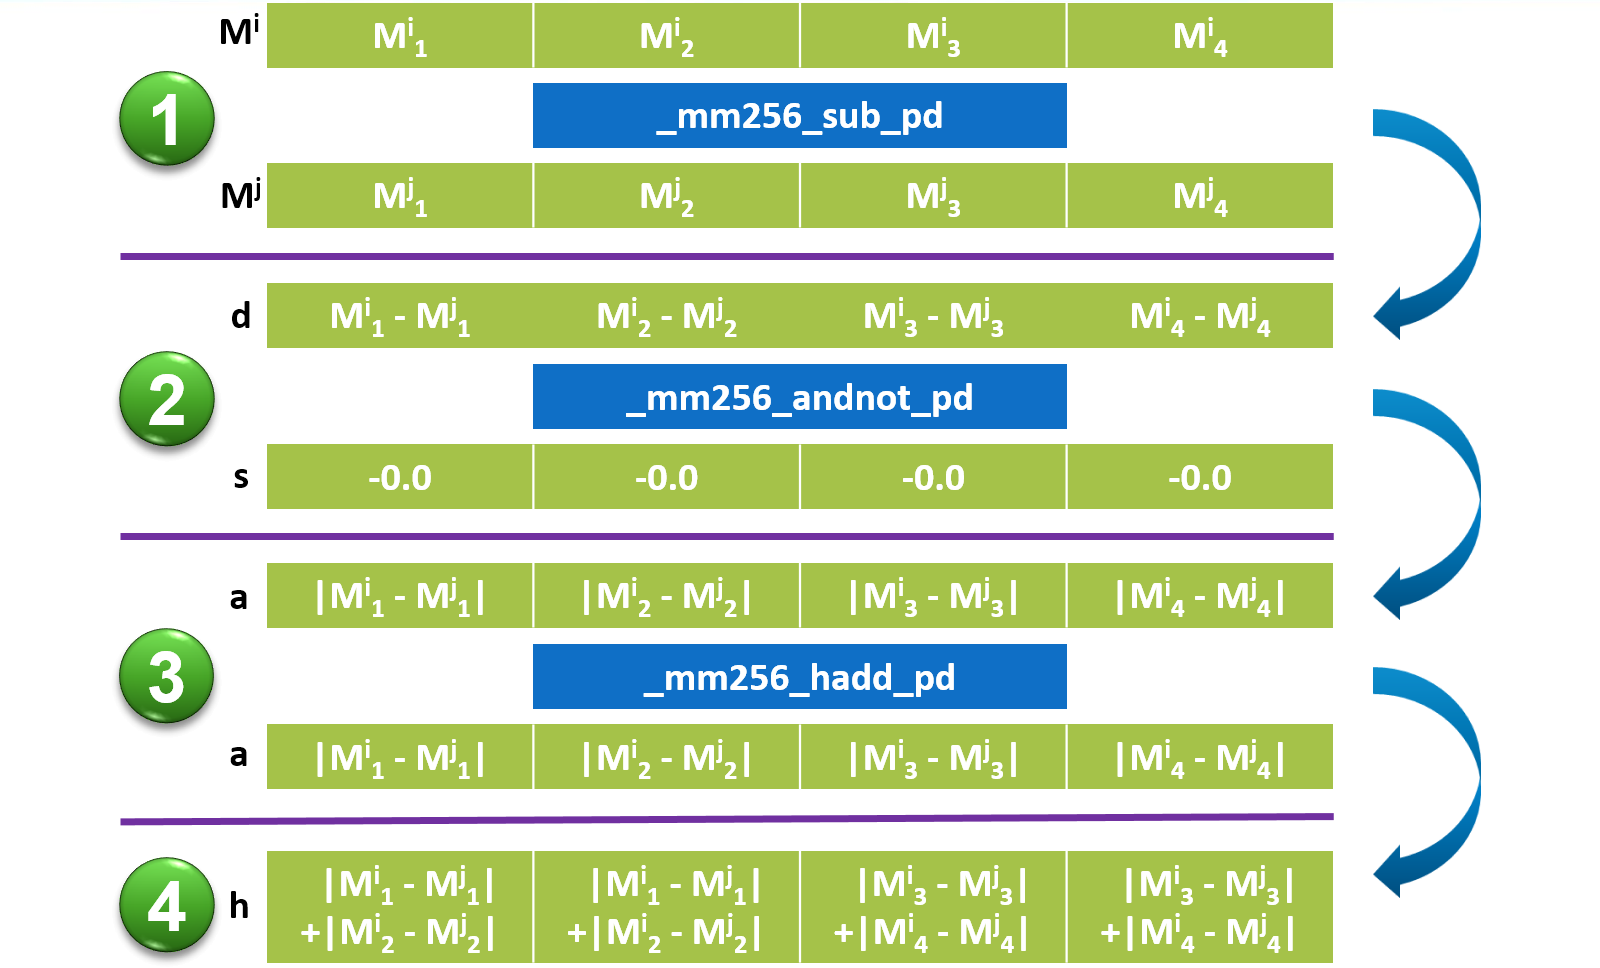
\includegraphics[width=\linewidth]{../usr/AVX.png}
\end{center}
\caption{AVX instructions used to compute USR or USRCAT scores.}
\label{usr:AVX}
\end{figure}

Our daemon supports a query ligand in either SDF, MOL2, XYZ, PDB or PDBQT format in one single job. Sample files in these formats are provided in the USR@istar web page. The parser on the server side is achieved by the C++ API of OpenBabel v2.3.2 \citep{968}, while the parser on the client side is our in-house JavaScript code. Moreover, our client side user interface features our WebGL visualizer iview \citep{1366} to realize interactive visualization of high-score hits.

\section{Results and discussion}

We selected 19 query ligands with different numbers of heavy atoms, spanning from 4 to 65 with a step size of 3 or 4 (Table \ref{usr:Queries}. HA: heavy atoms. MWT: molecular weight in Daltons. HBD: hydrogen bond donors. HBA: hydrogen bond acceptors. NRB: rotatable bonds).

\begin{table}
\caption{Molecular properties of the 19 query ligands.}
\label{usr:Queries}
\begin{tabular}{cccccc}
\hline
ZINC ID  & HA & MWT & HBD & HBA & NRB\\
\hline
06827693 &  4 &  60.008 & 0 &  3 &  0\\
03641271 &  7 & 103.101 & 4 &  4 &  0\\
00000882 & 10 & 135.130 & 3 &  5 &  0\\
03594299 & 13 & 176.243 & 4 &  3 &  1\\
01760831 & 16 & 206.244 & 0 &  1 &  0\\
00000163 & 19 & 277.771 & 0 &  2 &  2\\
00000931 & 22 & 314.796 & 2 &  4 &  1\\
00000706 & 25 & 332.335 & 0 &  5 &  0\\
00577115 & 28 & 382.449 & 1 &  1 &  5\\
03784182 & 31 & 411.521 & 0 &  3 &  4\\
00537755 & 35 & 476.591 & 2 &  4 &  7\\
33359785 & 39 & 536.653 & 4 & 10 &  3\\
53073961 & 42 & 588.552 & 1 &  6 & 10\\
34801951 & 46 & 650.698 & 4 & 12 &  7\\
29416466 & 49 & 671.863 & 7 & 11 & 13\\
08101127 & 53 & 751.991 & 0 &  8 & 14\\
08101051 & 57 & 806.987 & 4 & 14 &  9\\
85536932 & 60 & 835.944 & 3 & 15 & 15\\
96006018 & 65 & 914.187 & 3 & 14 &  6\\
\hline
\end{tabular}
\end{table}

\subsection{Matching ligands with different molecular sizes}

Table \ref{usr:Matches} lists the top five matching compounds of the 19 selected query ligands with different molecular sizes in terms of number of heavy atoms. Note that these query ligands were in their docked pose in PDBQT format generated by idock \citep{1362} when docked against cyclin-dependent kinase 2 (CDK2), a critical protein involved in the regulation of cell cycle transition, which will be detailed in Chapter \ref{cdk2}. In prospective applications, the advantage of using a docked pose as input is obvious because the matching output compounds are likely to exhibit geometrically similar shape, which could retain or even enhance the intermolecular interactions and thus the putative binding affinity. Not unexpectedly, sorting by USR or USRCAT score yielded different output. In 13 of the 19 cases, the top five matches by USR score were totally different from the top five matches by USRCAT score. Particularly, in 12 of these 13 cases, the query ligand had at least 25 heavy atoms. This may indicate that USR and USRCAT tend to prioritize distinct compounds when the query ligand is large. This result was to be expected because the larger the query ligand, the larger chemical and structural diversity of potential matching compounds.

\pagebreak
\begin{longtable}{cccccc}
\caption{Top 5 matches of 19 query ligands}
\label{usr:Matches}
\vspace{-3mm}
\\
\hline
input    & sorting & output & output   & USR   & USRCAT\\
ZINC ID  & method  & rank   & ZINC ID  & score & score\\
\hline
\endfirsthead
\multicolumn{6}{c}{\tablename\ \thetable\ -- \textit{Continued from previous page}} \\
\hline
input    & sorting & output & output   & USR   & USRCAT\\
ZINC ID  & method  & rank   & ZINC ID  & score & score\\
\hline
\endhead
06827693 & USR    & 1 & 06827693 & 0.99989084 & 0.93387099\\%5497dd76f33d108f178516ec
06827693 & USR    & 2 & 08214514 & 0.94435271 & 0.85958990\\
06827693 & USR    & 3 & 08101126 & 0.91583558 & 0.90090227\\
06827693 & USR    & 4 & 05224164 & 0.91323638 & 0.83597828\\
06827693 & USR    & 5 & 08034818 & 0.91124311 & 0.80893830\\
06827693 & USRCAT & 1 & 06827693 & 0.99989084 & 0.93387099\\%54978f1d61560ab5173f9630
06827693 & USRCAT & 2 & 08101126 & 0.91583558 & 0.90090227\\
06827693 & USRCAT & 3 & 01846598 & 0.82101487 & 0.86076010\\
06827693 & USRCAT & 4 & 08214514 & 0.94435271 & 0.85958990\\
06827693 & USRCAT & 5 & 04658552 & 0.77735039 & 0.85427671\\
\hline
03641271 & USR    & 1 & 19737051 & 0.98779656 & 0.82477674\\%5497de82f33d108f178516ed
03641271 & USR    & 2 & 34689286 & 0.98720924 & 0.82948216\\
03641271 & USR    & 3 & 04262127 & 0.98577986 & 0.83173477\\
03641271 & USR    & 4 & 05226936 & 0.98436293 & 0.77590893\\
03641271 & USR    & 5 & 05226942 & 0.98419217 & 0.77576925\\
03641271 & USRCAT & 1 & 04417022 & 0.90277096 & 0.95866631\\%54978f513e01d9b717d1826b
03641271 & USRCAT & 2 & 32296878 & 0.89128565 & 0.92383824\\
03641271 & USRCAT & 3 & 64033578 & 0.91094937 & 0.91829554\\
03641271 & USRCAT & 4 & 04658602 & 0.89124510 & 0.91780849\\
03641271 & USRCAT & 5 & 01666720 & 0.89345170 & 0.91692833\\
\hline
00000882 & USR    & 1 & 00000882 & 0.99992602 & 0.99993121\\%5497e0d861560ab5173f9632
00000882 & USR    & 2 & 26995176 & 0.99597115 & 0.80645548\\
00000882 & USR    & 3 & 72231352 & 0.99543539 & 0.82250290\\
00000882 & USR    & 4 & 82410931 & 0.99508429 & 0.81322159\\
00000882 & USR    & 5 & 01615910 & 0.99476961 & 0.85551400\\
00000882 & USRCAT & 1 & 00000882 & 0.99992602 & 0.99993121\\%54978f5af33d108f178516ea
00000882 & USRCAT & 2 & 08616408 & 0.99327569 & 0.98073897\\
00000882 & USRCAT & 3 & 03652180 & 0.98439837 & 0.93952496\\
00000882 & USRCAT & 4 & 18153302 & 0.97495298 & 0.93319108\\
00000882 & USRCAT & 5 & 13516924 & 0.99128475 & 0.92503209\\
\hline
03594299 & USR    & 1 & 03594299 & 0.99978454 & 0.99983624\\%5497e0e9c666488b17d07c85
03594299 & USR    & 2 & 86639023 & 0.94249238 & 0.56539305\\
03594299 & USR    & 3 & 23093521 & 0.94248914 & 0.67187858\\
03594299 & USR    & 4 & 63169716 & 0.94098603 & 0.56936544\\
03594299 & USR    & 5 & 23093522 & 0.93999049 & 0.67166081\\
03594299 & USRCAT & 1 & 03594299 & 0.99978454 & 0.99983624\\%54978f6486db148d17c90cc2
03594299 & USRCAT & 2 & 22219232 & 0.89835884 & 0.86306679\\
03594299 & USRCAT & 3 & 86051862 & 0.89218389 & 0.85055658\\
03594299 & USRCAT & 4 & 38532749 & 0.81227537 & 0.84324650\\
03594299 & USRCAT & 5 & 19796009 & 0.84131930 & 0.84309403\\
\hline
01760831 & USR    & 1 & 01760831 & 0.99987949 & 0.99989913\\%5497e2283e01d9b717d1826e
01760831 & USR    & 2 & 01709154 & 0.98699243 & 0.75851222\\
01760831 & USR    & 3 & 00971553 & 0.98535056 & 0.81526150\\
01760831 & USR    & 4 & 67730206 & 0.98262917 & 0.75827336\\
01760831 & USR    & 5 & 01681580 & 0.97753801 & 0.94530750\\
01760831 & USRCAT & 1 & 01760831 & 0.99987949 & 0.99989913\\%54978f6d3e01d9b717d1826c
01760831 & USRCAT & 2 & 01681580 & 0.97753801 & 0.94530750\\
01760831 & USRCAT & 3 & 02510715 & 0.89837623 & 0.91571639\\
01760831 & USRCAT & 4 & 01555275 & 0.88135318 & 0.90937875\\
01760831 & USRCAT & 5 & 39255067 & 0.89111121 & 0.90652744\\
\hline
00000163 & USR    & 1 & 00000163 & 0.96426028 & 0.95981456\\%5497e23661560ab5173f9633
00000163 & USR    & 2 & 95003095 & 0.96059429 & 0.46005568\\
00000163 & USR    & 3 & 94998736 & 0.95953442 & 0.45932022\\
00000163 & USR    & 4 & 93855398 & 0.95647154 & 0.56896132\\
00000163 & USR    & 5 & 94468575 & 0.94929677 & 0.52144044\\
00000163 & USRCAT & 1 & 00000163 & 0.96426028 & 0.95981456\\%54978f7bc4c24aa0172a679d
00000163 & USRCAT & 2 & 12336856 & 0.88870156 & 0.87618989\\
00000163 & USRCAT & 3 & 72196442 & 0.85417800 & 0.86199583\\
00000163 & USRCAT & 4 & 03830577 & 0.89135269 & 0.84555906\\
00000163 & USRCAT & 5 & 71767467 & 0.79282467 & 0.84492369\\
\hline
00000931 & USR    & 1 & 33693318 & 0.96997742 & 0.78246622\\%5497e241de44fb911775c97a
00000931 & USR    & 2 & 00000931 & 0.96952854 & 0.98807569\\
00000931 & USR    & 3 & 66774020 & 0.96744933 & 0.69240859\\
00000931 & USR    & 4 & 66773996 & 0.96728672 & 0.70565997\\
00000931 & USR    & 5 & 66546099 & 0.96669849 & 0.55832601\\
00000931 & USRCAT & 1 & 00000931 & 0.96952854 & 0.98807569\\%54978f863e01d9b717d1826d
00000931 & USRCAT & 2 & 05284765 & 0.89184694 & 0.84417333\\
00000931 & USRCAT & 3 & 02193124 & 0.93922432 & 0.83616846\\
00000931 & USRCAT & 4 & 36020480 & 0.88785134 & 0.82437481\\
00000931 & USRCAT & 5 & 05011019 & 0.90642740 & 0.82042605\\
\hline
00000706 & USR    & 1 & 65405747 & 0.95996452 & 0.44442734\\%5497e24d61560ab5173f9634
00000706 & USR    & 2 & 40647363 & 0.95682962 & 0.50111399\\
00000706 & USR    & 3 & 93828780 & 0.95053992 & 0.40343405\\
00000706 & USR    & 4 & 72255543 & 0.95023716 & 0.54229924\\
00000706 & USR    & 5 & 00408247 & 0.94828659 & 0.51394696\\
00000706 & USRCAT & 1 & 80448655 & 0.87617333 & 0.83086022\\%54978f8fc666488b17d07c84
00000706 & USRCAT & 2 & 78886065 & 0.77618234 & 0.82713956\\
00000706 & USRCAT & 3 & 93775002 & 0.73152053 & 0.82414472\\
00000706 & USRCAT & 4 & 78886066 & 0.76913264 & 0.82370563\\
00000706 & USRCAT & 5 & 78700739 & 0.89428224 & 0.81951128\\
\hline
00577115 & USR    & 1 & 68658377 & 0.95057414 & 0.39005121\\%5497e2573e01d9b717d1826f
00577115 & USR    & 2 & 69389189 & 0.94579839 & 0.35499414\\
00577115 & USR    & 3 & 89143595 & 0.94491604 & 0.46345807\\
00577115 & USR    & 4 & 78399755 & 0.94491250 & 0.45419415\\
00577115 & USR    & 5 & 83027211 & 0.94480002 & 0.34078650\\
00577115 & USRCAT & 1 & 22657173 & 0.61248204 & 0.75399074\\%54978f988181019317571804
00577115 & USRCAT & 2 & 01550499 & 0.56107197 & 0.74185012\\
00577115 & USRCAT & 3 & 11678289 & 0.55772743 & 0.73271990\\
00577115 & USRCAT & 4 & 11662947 & 0.82521725 & 0.72450314\\
00577115 & USRCAT & 5 & 08474264 & 0.84212073 & 0.72433086\\
\hline
03784182 & USR    & 1 & 67249641 & 0.94940522 & 0.45316801\\%5497e26186db148d17c90cc3
03784182 & USR    & 2 & 79160658 & 0.94444038 & 0.37397556\\
03784182 & USR    & 3 & 66798033 & 0.94393213 & 0.41624736\\
03784182 & USR    & 4 & 78080377 & 0.94104867 & 0.41947726\\
03784182 & USR    & 5 & 44148945 & 0.93967079 & 0.39586261\\
03784182 & USRCAT & 1 & 03784182 & 0.77235330 & 0.83985811\\%54978fa2de44fb911775c974
03784182 & USRCAT & 2 & 71789431 & 0.74342618 & 0.80805432\\
03784182 & USRCAT & 3 & 93106652 & 0.73942307 & 0.66665953\\
03784182 & USRCAT & 4 & 93106649 & 0.73848385 & 0.66623719\\
03784182 & USRCAT & 5 & 90800223 & 0.64094384 & 0.66486802\\
\hline
00537755 & USR    & 1 & 33077240 & 0.92816370 & 0.46838130\\%5497e26bc666488b17d07c86
00537755 & USR    & 2 & 71880803 & 0.92703459 & 0.44320682\\
00537755 & USR    & 3 & 10246617 & 0.92144736 & 0.47914766\\
00537755 & USR    & 4 & 34759207 & 0.91737385 & 0.43123165\\
00537755 & USR    & 5 & 03223873 & 0.91734806 & 0.50177117\\
00537755 & USRCAT & 1 & 65623842 & 0.82911423 & 0.73050138\\%54978fab8181019317571805
00537755 & USRCAT & 2 & 65623840 & 0.82920422 & 0.73043065\\
00537755 & USRCAT & 3 & 65623844 & 0.84434115 & 0.72502994\\
00537755 & USRCAT & 4 & 65623838 & 0.84429533 & 0.72498612\\
00537755 & USRCAT & 5 & 91738997 & 0.80098542 & 0.72414875\\
\hline
33359785 & USR    & 1 & 35770975 & 0.93307793 & 0.35822866\\%5497e2783e01d9b717d18270
33359785 & USR    & 2 & 72004193 & 0.93114334 & 0.38182298\\
33359785 & USR    & 3 & 33435896 & 0.92965520 & 0.33894654\\
33359785 & USR    & 4 & 09254874 & 0.92781816 & 0.40359101\\
33359785 & USR    & 5 & 12807677 & 0.92642912 & 0.35213376\\
33359785 & USRCAT & 1 & 79055171 & 0.84112415 & 0.71794128\\%54978fb58181019317571806
33359785 & USRCAT & 2 & 71923062 & 0.73844740 & 0.71181372\\
33359785 & USRCAT & 3 & 77341431 & 0.75924711 & 0.70930088\\
33359785 & USRCAT & 4 & 77341441 & 0.75921732 & 0.70927376\\
33359785 & USRCAT & 5 & 69046249 & 0.70287350 & 0.70695212\\
\hline
53073961 & USR    & 1 & 03280771 & 0.89422462 & 0.55998626\\%5497e2823e01d9b717d18271
53073961 & USR    & 2 & 12509920 & 0.89370657 & 0.48547850\\
53073961 & USR    & 3 & 34899971 & 0.89334569 & 0.59114533\\
53073961 & USR    & 4 & 15730136 & 0.89292055 & 0.47162568\\
53073961 & USR    & 5 & 09451077 & 0.89287846 & 0.40216378\\
53073961 & USRCAT & 1 & 20677274 & 0.82865029 & 0.73844702\\%54978fbede44fb911775c975
53073961 & USRCAT & 2 & 08916625 & 0.80980780 & 0.72773540\\
53073961 & USRCAT & 3 & 02110104 & 0.80092701 & 0.72556402\\
53073961 & USRCAT & 4 & 20685629 & 0.84494018 & 0.71625164\\
53073961 & USRCAT & 5 & 53064465 & 0.81539807 & 0.71344270\\
\hline
34801951 & USR    & 1 & 09813531 & 0.86662080 & 0.49260706\\%5497e28cf33d108f178516ee
34801951 & USR    & 2 & 10120418 & 0.85012639 & 0.48564947\\
34801951 & USR    & 3 & 22633339 & 0.84690548 & 0.32109534\\
34801951 & USR    & 4 & 09942653 & 0.83253562 & 0.41993991\\
34801951 & USR    & 5 & 09016590 & 0.83239022 & 0.44123198\\
34801951 & USRCAT & 1 & 09730878 & 0.78365470 & 0.65931372\\%54978fcade44fb911775c976
34801951 & USRCAT & 2 & 02952637 & 0.69990120 & 0.63865229\\
34801951 & USRCAT & 3 & 03066292 & 0.79377130 & 0.63427123\\
34801951 & USRCAT & 4 & 63600618 & 0.78591726 & 0.62978556\\
34801951 & USRCAT & 5 & 02171971 & 0.81658623 & 0.62773804\\
\hline
29416466 & USR    & 1 & 63514587 & 0.91665219 & 0.46731155\\%5497e29761560ab5173f9635
29416466 & USR    & 2 & 40292843 & 0.91468903 & 0.47087614\\
29416466 & USR    & 3 & 40293083 & 0.91077708 & 0.45683873\\
29416466 & USR    & 4 & 22052805 & 0.90502904 & 0.50124716\\
29416466 & USR    & 5 & 22052817 & 0.90013261 & 0.56632489\\
29416466 & USRCAT & 1 & 13389101 & 0.77024906 & 0.69218386\\%54978fd5de44fb911775c977
29416466 & USRCAT & 2 & 67741752 & 0.71934043 & 0.68237936\\
29416466 & USRCAT & 3 & 67769739 & 0.71092297 & 0.67849718\\
29416466 & USRCAT & 4 & 27016688 & 0.75586732 & 0.66575518\\
29416466 & USRCAT & 5 & 27016682 & 0.73442306 & 0.66531265\\
\hline
08101127 & USR    & 1 & 40253466 & 0.82049130 & 0.45823208\\%5497e2a1f33d108f178516ef
08101127 & USR    & 2 & 40251780 & 0.81389665 & 0.44709474\\
08101127 & USR    & 3 & 40253347 & 0.81270120 & 0.45688630\\
08101127 & USR    & 4 & 40252264 & 0.81007384 & 0.43212674\\
08101127 & USR    & 5 & 40252260 & 0.80935988 & 0.42814493\\
08101127 & USRCAT & 1 & 40204804 & 0.70216986 & 0.61769941\\%54978fdede44fb911775c978
08101127 & USRCAT & 2 & 40203918 & 0.72134056 & 0.61467790\\
08101127 & USRCAT & 3 & 40198912 & 0.75040459 & 0.61092978\\
08101127 & USRCAT & 4 & 19788980 & 0.67787440 & 0.60600169\\
08101127 & USRCAT & 5 & 40203919 & 0.72535625 & 0.60578330\\
\hline
08101051 & USR    & 1 & 34906112 & 0.81662557 & 0.38601073\\%5497e2b461560ab5173f9636
08101051 & USR    & 2 & 12790633 & 0.81216532 & 0.38263829\\
08101051 & USR    & 3 & 34905308 & 0.81088357 & 0.37345643\\
08101051 & USR    & 4 & 34906092 & 0.80499926 & 0.37499018\\
08101051 & USR    & 5 & 22623297 & 0.80282387 & 0.42624504\\
08101051 & USRCAT & 1 & 91742856 & 0.62507638 & 0.63946406\\%54978fe761560ab5173f9631
08101051 & USRCAT & 2 & 63634534 & 0.68412199 & 0.63451306\\
08101051 & USRCAT & 3 & 63634530 & 0.66760438 & 0.63182588\\
08101051 & USRCAT & 4 & 12530576 & 0.59249267 & 0.62763900\\
08101051 & USRCAT & 5 & 08872621 & 0.63481592 & 0.62422077\\
\hline
85536932 & USR    & 1 & 38491099 & 0.87113381 & 0.54465979\\%5497e2bd61560ab5173f9637
85536932 & USR    & 2 & 33767419 & 0.86880460 & 0.51486740\\
85536932 & USR    & 3 & 12304689 & 0.86865297 & 0.56751118\\
85536932 & USR    & 4 & 00903819 & 0.85511867 & 0.44597602\\
85536932 & USR    & 5 & 12706271 & 0.85465720 & 0.44716140\\
85536932 & USRCAT & 1 & 63386406 & 0.72871316 & 0.62348129\\%54978fefde44fb911775c979
85536932 & USRCAT & 2 & 14232016 & 0.70572357 & 0.61247207\\
85536932 & USRCAT & 3 & 38573815 & 0.72269606 & 0.61188087\\
85536932 & USRCAT & 4 & 09713729 & 0.78048080 & 0.60555170\\
85536932 & USRCAT & 5 & 26998174 & 0.74923801 & 0.59966269\\
\hline
96006018 & USR    & 1 & 40200504 & 0.83259667 & 0.31658414\\%5497e2c8f33d108f178516f0
96006018 & USR    & 2 & 35402146 & 0.79559059 & 0.35874467\\
96006018 & USR    & 3 & 10462892 & 0.78614715 & 0.34836142\\
96006018 & USR    & 4 & 09693915 & 0.78488061 & 0.33538157\\
96006018 & USR    & 5 & 40206470 & 0.78111193 & 0.30224723\\
96006018 & USRCAT & 1 & 77320087 & 0.65583149 & 0.61433137\\%54978ff7c4c24aa0172a679e
96006018 & USRCAT & 2 & 31392738 & 0.64614083 & 0.58921551\\
96006018 & USRCAT & 3 & 04536260 & 0.60279466 & 0.57727754\\
96006018 & USRCAT & 4 & 89960170 & 0.47860515 & 0.57257619\\
96006018 & USRCAT & 5 & 66730926 & 0.48114189 & 0.56721396\\
\hline
\end{longtable}

Figures \ref{usr:ZINC00000706}, \ref{usr:ZINC00577115}, \ref{usr:ZINC03784182}, \ref{usr:ZINC00537755} and \ref{usr:ZINC33359785} plot the 2D diagrams of five query ligands, which are ZINC00000706, ZINC00577115, ZINC03784182, ZINC00537755 and ZINC33359785, respectively. These five query ligands were selected for visualization because their molecular weight (Table \ref{usr:Queries}) is in the range of candidate leads, so they are of high chance of being selected as query ligands in real case studies. Note that the output compounds were not structurally aligned to the query.

\begin{figure}
\centering
\subfloat[Query]
{
  \includegraphics[width=0.33\linewidth]{../usr/1GZ8/00000706/ZINC00000706.png}
}
\subfloat[USR rank 1.]
{
  \includegraphics[width=0.33\linewidth]{../usr/1GZ8/00000706/usr/ZINC65405747.png}
}
\subfloat[USR rank 2.]
{
  \includegraphics[width=0.33\linewidth]{../usr/1GZ8/00000706/usr/ZINC40647363.png}
}
\\
\subfloat[USR rank 3.]
{
  \includegraphics[width=0.33\linewidth]{../usr/1GZ8/00000706/usr/ZINC93828780.png}
}
\subfloat[USR rank 4.]
{
  \includegraphics[width=0.33\linewidth]{../usr/1GZ8/00000706/usr/ZINC72255543.png}
}
\subfloat[USR rank 5.]
{
  \includegraphics[width=0.33\linewidth]{../usr/1GZ8/00000706/usr/ZINC00408247.png}
}
\\
\subfloat[Query]
{
  \includegraphics[width=0.33\linewidth]{../usr/1GZ8/00000706/ZINC00000706.png}
}
\subfloat[USRCAT rank 1.]
{
  \includegraphics[width=0.33\linewidth]{../usr/1GZ8/00000706/usrcat/ZINC80448655.png}
}
\subfloat[USRCAT rank 2.]
{
  \includegraphics[width=0.33\linewidth]{../usr/1GZ8/00000706/usrcat/ZINC78886065.png}
}
\\
\subfloat[USRCAT rank 3.]
{
  \includegraphics[width=0.33\linewidth]{../usr/1GZ8/00000706/usrcat/ZINC93775002.png}
}
\subfloat[USRCAT rank 4.]
{
  \includegraphics[width=0.33\linewidth]{../usr/1GZ8/00000706/usrcat/ZINC78886066.png}
}
\subfloat[USRCAT rank 5.]
{
  \includegraphics[width=0.33\linewidth]{../usr/1GZ8/00000706/usrcat/ZINC78700739.png}
}
\caption{Top 5 matching compounds for ZINC00000706 (a \& g) using USR (b to f) or USRCAT (h to l).}
\label{usr:ZINC00000706}
\end{figure}

\begin{figure}
\centering
\subfloat[Query]
{
  \includegraphics[width=0.33\linewidth]{../usr/1GZ8/00577115/ZINC00577115.png}
}
\subfloat[USR rank 1.]
{
  \includegraphics[width=0.33\linewidth]{../usr/1GZ8/00577115/usr/ZINC68658377.png}
}
\subfloat[USR rank 2.]
{
  \includegraphics[width=0.33\linewidth]{../usr/1GZ8/00577115/usr/ZINC69389189.png}
}
\\
\subfloat[USR rank 3.]
{
  \includegraphics[width=0.33\linewidth]{../usr/1GZ8/00577115/usr/ZINC89143595.png}
}
\subfloat[USR rank 4.]
{
  \includegraphics[width=0.33\linewidth]{../usr/1GZ8/00577115/usr/ZINC78399755.png}
}
\subfloat[USR rank 5.]
{
  \includegraphics[width=0.33\linewidth]{../usr/1GZ8/00577115/usr/ZINC83027211.png}
}
\\
\subfloat[Query]
{
  \includegraphics[width=0.33\linewidth]{../usr/1GZ8/00577115/ZINC00577115.png}
}
\subfloat[USRCAT rank 1.]
{
  \includegraphics[width=0.33\linewidth]{../usr/1GZ8/00577115/usrcat/ZINC22657173.png}
}
\subfloat[USRCAT rank 2.]
{
  \includegraphics[width=0.33\linewidth]{../usr/1GZ8/00577115/usrcat/ZINC01550499.png}
}
\\
\subfloat[USRCAT rank 3.]
{
  \includegraphics[width=0.33\linewidth]{../usr/1GZ8/00577115/usrcat/ZINC11678289.png}
}
\subfloat[USRCAT rank 4.]
{
  \includegraphics[width=0.33\linewidth]{../usr/1GZ8/00577115/usrcat/ZINC11662947.png}
}
\subfloat[USRCAT rank 5.]
{
  \includegraphics[width=0.33\linewidth]{../usr/1GZ8/00577115/usrcat/ZINC08474264.png}
}
\caption{Top 5 matching compounds for ZINC00577115 (a \& g) using USR (b to f) or USRCAT (h to l).}
\label{usr:ZINC00577115}
\end{figure}

\begin{figure}
\centering
\subfloat[Query]
{
  \includegraphics[width=0.33\linewidth]{../usr/1GZ8/03784182/ZINC03784182.png}
}
\subfloat[USR rank 1.]
{
  \includegraphics[width=0.33\linewidth]{../usr/1GZ8/03784182/usr/ZINC67249641.png}
}
\subfloat[USR rank 2.]
{
  \includegraphics[width=0.33\linewidth]{../usr/1GZ8/03784182/usr/ZINC79160658.png}
}
\\
\subfloat[USR rank 3.]
{
  \includegraphics[width=0.33\linewidth]{../usr/1GZ8/03784182/usr/ZINC66798033.png}
}
\subfloat[USR rank 4.]
{
  \includegraphics[width=0.33\linewidth]{../usr/1GZ8/03784182/usr/ZINC78080377.png}
}
\subfloat[USR rank 5.]
{
  \includegraphics[width=0.33\linewidth]{../usr/1GZ8/03784182/usr/ZINC44148945.png}
}
\\
\subfloat[Query]
{
  \includegraphics[width=0.33\linewidth]{../usr/1GZ8/03784182/ZINC03784182.png}
}
\subfloat[USRCAT rank 1.]
{
  \includegraphics[width=0.33\linewidth]{../usr/1GZ8/03784182/usrcat/ZINC03784182.png}
}
\subfloat[USRCAT rank 2.]
{
  \includegraphics[width=0.33\linewidth]{../usr/1GZ8/03784182/usrcat/ZINC71789431.png}
}
\\
\subfloat[USRCAT rank 3.]
{
  \includegraphics[width=0.33\linewidth]{../usr/1GZ8/03784182/usrcat/ZINC93106652.png}
}
\subfloat[USRCAT rank 4.]
{
  \includegraphics[width=0.33\linewidth]{../usr/1GZ8/03784182/usrcat/ZINC93106649.png}
}
\subfloat[USRCAT rank 5.]
{
  \includegraphics[width=0.33\linewidth]{../usr/1GZ8/03784182/usrcat/ZINC90800223.png}
}
\caption{Top 5 matching compounds for ZINC03784182 (a \& g) using USR (b to f) or USRCAT (h to l).}
\label{usr:ZINC03784182}
\end{figure}

\begin{figure}
\centering
\subfloat[Query]
{
  \includegraphics[width=0.33\linewidth]{../usr/1GZ8/00537755/ZINC00537755.png}
}
\subfloat[USR rank 1.]
{
  \includegraphics[width=0.33\linewidth]{../usr/1GZ8/00537755/usr/ZINC33077240.png}
}
\subfloat[USR rank 2.]
{
  \includegraphics[width=0.33\linewidth]{../usr/1GZ8/00537755/usr/ZINC71880803.png}
}
\\
\subfloat[USR rank 3.]
{
  \includegraphics[width=0.33\linewidth]{../usr/1GZ8/00537755/usr/ZINC10246617.png}
}
\subfloat[USR rank 4.]
{
  \includegraphics[width=0.33\linewidth]{../usr/1GZ8/00537755/usr/ZINC34759207.png}
}
\subfloat[USR rank 5.]
{
  \includegraphics[width=0.33\linewidth]{../usr/1GZ8/00537755/usr/ZINC03223873.png}
}
\\
\subfloat[Query]
{
  \includegraphics[width=0.33\linewidth]{../usr/1GZ8/00537755/ZINC00537755.png}
}
\subfloat[USRCAT rank 1.]
{
  \includegraphics[width=0.33\linewidth]{../usr/1GZ8/00537755/usrcat/ZINC65623842.png}
}
\subfloat[USRCAT rank 2.]
{
  \includegraphics[width=0.33\linewidth]{../usr/1GZ8/00537755/usrcat/ZINC65623840.png}
}
\\
\subfloat[USRCAT rank 3.]
{
  \includegraphics[width=0.33\linewidth]{../usr/1GZ8/00537755/usrcat/ZINC65623844.png}
}
\subfloat[USRCAT rank 4.]
{
  \includegraphics[width=0.33\linewidth]{../usr/1GZ8/00537755/usrcat/ZINC65623838.png}
}
\subfloat[USRCAT rank 5.]
{
  \includegraphics[width=0.33\linewidth]{../usr/1GZ8/00537755/usrcat/ZINC91738997.png}
}
\caption{Top 5 matching compounds for ZINC00537755 (a \& g) using USR (b to f) or USRCAT (h to l).}
\label{usr:ZINC00537755}
\end{figure}

\begin{figure}
\centering
\subfloat[Query]
{
  \includegraphics[width=0.33\linewidth]{../usr/1GZ8/33359785/ZINC33359785.png}
}
\subfloat[USR rank 1.]
{
  \includegraphics[width=0.33\linewidth]{../usr/1GZ8/33359785/usr/ZINC35770975.png}
}
\subfloat[USR rank 2.]
{
  \includegraphics[width=0.33\linewidth]{../usr/1GZ8/33359785/usr/ZINC72004193.png}
}
\\
\subfloat[USR rank 3.]
{
  \includegraphics[width=0.33\linewidth]{../usr/1GZ8/33359785/usr/ZINC33435896.png}
}
\subfloat[USR rank 4.]
{
  \includegraphics[width=0.33\linewidth]{../usr/1GZ8/33359785/usr/ZINC09254874.png}
}
\subfloat[USR rank 5.]
{
  \includegraphics[width=0.33\linewidth]{../usr/1GZ8/33359785/usr/ZINC12807677.png}
}
\\
\subfloat[Query]
{
  \includegraphics[width=0.33\linewidth]{../usr/1GZ8/33359785/ZINC33359785.png}
}
\subfloat[USRCAT rank 1.]
{
  \includegraphics[width=0.33\linewidth]{../usr/1GZ8/33359785/usrcat/ZINC79055171.png}
}
\subfloat[USRCAT rank 2.]
{
  \includegraphics[width=0.33\linewidth]{../usr/1GZ8/33359785/usrcat/ZINC71923062.png}
}
\\
\subfloat[USRCAT rank 3.]
{
  \includegraphics[width=0.33\linewidth]{../usr/1GZ8/33359785/usrcat/ZINC77341431.png}
}
\subfloat[USRCAT rank 4.]
{
  \includegraphics[width=0.33\linewidth]{../usr/1GZ8/33359785/usrcat/ZINC77341441.png}
}
\subfloat[USRCAT rank 5.]
{
  \includegraphics[width=0.33\linewidth]{../usr/1GZ8/33359785/usrcat/ZINC69046249.png}
}
\caption{Top 5 matching compounds for ZINC33359785 (a \& g) using USR (b to f) or USRCAT (h to l).}
\label{usr:ZINC33359785}
\end{figure}

Next, we examined the capability of ranking high the particular compound in the output with an identical ZINC ID as the input query. Apparently, such recovery test requires that the query compound must be present in the molecular database, although it can be in a different pose. Out of the 19 query ligands, 9 satisfied this requirement (Table \ref{usr:RecoveryRate}). Note again that the query ligands were in their docked pose while the compounds in the molecular database were in their low energy pose, therefore the corresponding compound with an identical ZINC ID as the input query was not always guaranteed to be ranked the first in the output. Interestingly, the recovery rate seemed to correlate with NRB (number of rotatable bonds). When NRB was zero, both USR and USRCAT ranked the input compound the highest in the output. When NRB was 1 or 2, the recovery rate started to drop slightly for USR. When NRB was equal to or beyond 4, both methods had difficulty in prioritizing the input compound in the output. This observation was to be expected because USR or USRCAT is dependent on torsions, though independent of position and orientation. When a compound has a NRB of zero, there is only one possible conformation, so the docked pose of the query must be conformationally equivalent to the original pose present in the molecular database. On the other hand, when a compound has a large NRB, there is a high chance that the docked pose and the original pose differ remarkably in their torsions, and so are their encoded features.

\begin{table}
\caption{}
\label{usr:RecoveryRate}
\begin{tabular}{cccc}
\hline
input    &     & USR rank of the     & USRCAT rank of the
ZINC ID  & NRB & same input compound & same input compound\\
\hline
06827693 &   0 &     1 &     1\\
00000882 &   0 &     1 &     1\\
01760831 &   0 &     1 &     1\\
03594299 &   1 &     1 &     1\\
00000931 &   1 &     2 &     1\\
00000163 &   2 &     1 &     1\\
03784182 &   4 & >1000 &     1\\
00577115 &   5 & >1000 & >1000\\
00537755 &   7 & >1000 & >1000\\
\hline
\end{tabular}
\end{table}

\subsection{Impact of file format on pharmacophoric subset classification}

It was anticipated that the same query ligand should yield identical output regardless of its input file format, be it sdf, mol2 or pdbqt. Surprisingly, we found that this was not necessarily the case. We used as an example ZINC00537755 in its low energy pose (Figure \ref{usr:ZINC00537755-N3}) rather than in its docked pose in order to retrieve a USR score and a USRCAT score of exactly one. When the query ligand was in pdbqt format, the same format used to encode the molecular database, the corresponding output compound had USR and USRCAT scores of exactly one and hence was ranked the first. Nevertheless, for the same query, if the format was changed to sdf or mol2, the corresponding output compound turned out to have a USR score of 0.99984619 and a USRCAT score of just 0.81023940, though it was still ranked the first (Table \ref{usr:ZINC00537755-Top5}).

\begin{figure}
\centering
\includegraphics[width=\linewidth]{../usr/ZINC00537755-N3.png}
\caption{ZINC00537755 with the N3 atom labeled.}
\label{usr:ZINC00537755-N3}
\end{figure}

\begin{table}
\caption{Top 5 matches of ZINC00537755 in pdbqt or sdf/mol2 format.}
\label{usr:ZINC00537755-Top5}
\begin{tabular}{cccccc}
\hline
input    & input  & output & output   & USR   & USRCAT\\
ZINC ID  & format & rank   & ZINC ID  & score & score\\
\hline
00537755 & pdbqt    & 1 & 00537755 & 1.00000000 & 1.00000000\\
00537755 & pdbqt    & 2 & 91686384 & 0.81962803 & 0.66995207\\
00537755 & pdbqt    & 3 & 09254146 & 0.80012011 & 0.66812359\\
00537755 & pdbqt    & 4 & 22804726 & 0.76476137 & 0.66203173\\
00537755 & pdbqt    & 5 & 22919990 & 0.69273531 & 0.66197772\\
00537755 & sdf/mol2 & 1 & 00537755 & 0.99984619 & 0.81023940\\
00537755 & sdf/mol2 & 2 & 89286333 & 0.71411555 & 0.65628724\\
00537755 & sdf/mol2 & 3 & 89286335 & 0.71272183 & 0.65581047\\
00537755 & sdf/mol2 & 4 & 26008225 & 0.85084668 & 0.65553656\\
00537755 & sdf/mol2 & 5 & 67878453 & 0.64157793 & 0.65528239\\
\hline
\end{tabular}
\end{table}

The large deviation in USRCAT score from an expected value of one attracted our attention. After careful investigations, we were surprised to find that the N3 atom, connected to a polar hydrogen and therefore supposed to be a hydrogen bond donor (Figure \ref{usr:ZINC00537755-N3}), failed to be recognized so in the SMARTS matching operation by OpenBabel \citep{968} when the query was in pdbqt format. This certainly had a great impact on the score of USRCAT, which requires classification of atoms into five predefined pharmacophoric subsets prior to moment calculation.

Such misclassification of a certain pharmacophoric subset other than heavy atoms should not affect USR score, which merely replies on heavy atoms to calculate the features. The USR score for the query in sdf/mol2 format was somewhat less than one because the coordinates in sdf/mol2 format have 4 decimal digits, whereas those in pdbqt format have 3 decimal digits.

\subsection{Execution time}

For the 19 selected queries, we inserted additional code to the daemon to record their execution time on the server equipped with Intel Xeon W3520 and 16GB ECC DDR3. Their execution times were averaged to 167 seconds and were quite consistent with a small standard deviation across 19 query ligands (Table \ref{usr:ExecutionTime}) regardless of their molecular size in terms of number of heavy atoms, molecular weight, or number of rotatable bonds.

\begin{table}
\caption{Execution time in seconds of the 19 queries when the USRCAT features are loaded \textit{ad hoc} or in advance.}
\label{usr:ExecutionTime}
\begin{tabular}{ccc}
\hline
ZINC ID  & \textit{ad hoc} (s) & in advance (s)\\
\hline
06827693 & 171 & 34\\
03641271 & 165 & 20\\
00000882 & 172 & 29\\
03594299 & 173 & 30\\
01760831 & 172 & 30\\
00000163 & 173 & 29\\
00000931 & 164 & 31\\
00000706 & 163 & 29\\
00577115 & 163 & 30\\
03784182 & 165 & 30\\
00537755 & 167 & 32\\
33359785 & 166 & 28\\
53073961 & 167 & 31\\
34801951 & 165 & 31\\
29416466 & 166 & 32\\
08101127 & 161 & 27\\
08101051 & 164 & 31\\
85536932 & 164 & 30\\
96006018 & 164 & 30\\
\hline
 Average & 167 & 30\\
 Std dev &   4 &  3\\
\hline
\end{tabular}
\end{table}

We further measured to what extent preloading the precalculated USRCAT features of the 23 million compounds would help shorten the query time. The size of entire features is $8B*60*23M=10GB$. These features can be loaded from hard disk \textit{ad hoc} or in advance. In the latter case, there are two additional one-off steps, memory allocation and file reading. Memory allocation took 5 seconds, which could be longer in case of insufficient free memory and therefore requirement of spare capacity from hard disk swapping. File reading from hard disk took another 149 seconds. Subsequently during USR and USRCAT score calculation, it required just 30 seconds to complete a query on average, compared to 167 seconds when the features were loaded \textit{ad hoc}. In other words, the pairwise similarity score computation accounted only for 18\% (=30/167) of the matching time, while the majority 82\% time was spent in file reading. This suggests that job execution is IO bound, hence deploying the daemon on a server with sufficient memory helps to reduce query time significantly.

\section{Conclusions}

Searching for compounds that resemble the shape of a given query molecule is a widely seen yet daunting problem in ligand-based virtual screening \citep{1332,1380,1281,1504,1502} and macromolecular target prediction \citep{1407,1408,1402}. The USR-like methods \citep{1379,1338,1331} represent an entirely new class of non-superposition algorithms that effectively capture the molecular shape information independent of spatial position and orientation. They circumvent the requirement of structural alignment and demonstrate outstanding computational efficiency with respect to superposition-based methods \citep{1440,887,1439}.

In this study we reviewed the traditional USR method \citep{1379} and its various extensions \citep{1333,1436,1437,1334,1335,1337,1338,1331,1407,1408}, as well as their applications, both retrospective \citep{1332,1331} and prospective \citep{1505,1380,1281,1504,1502,1615}. We highlighted the pros and cons of three web servers \citep{1436,1437,1408} which use USR variants as their underlying methods. Consequently, to address the existing constraints, we designed our pragmatic implementation of USR \citep{1379} and USRCAT \citep{1331} on istar \citep{1362} and explained its methodological advancement in terms of functionality, usability, and efficiency.

First and foremost, our molecular database was populated with more than 23 million small and diverse molecules that are collected from the ZINC database \citep{532,1178} and thus possibly commercially available to purchase for subsequent biological assays. We also proposed to generate low-energy conformers that are likely to occur in nature. The reason why a molecular database should be populated with multiple conformers of each flexible compound is to reduce the possibility of missing compounds with similar shape to the query. We would use RDKit and the postprocessing algorithm suggested in \citep{1127} for the conformer generation task in the near future. The USR and USRCAT features of these 23 million compounds were precalculated, which is an one-off exercise.

Second, we estimated the storage size of all descriptors across the entire database, and suggested two approaches, i.e. preloading all descriptors at once and loading them chunk by chunk, and analyzed their theoretical execution time. Based on the time analysis, we exploited three levels of parallelism, which map multiple jobs to multiple servers, multiple queries to multiple CPU cores, and multiple descriptors to multiple registers, respectively, to fully utilize all available computational resources so as to accelerate job execution. Notably, we described a novel AVX implementation of sum of absolute differences to calculate the USR or USRCAT scores between two moment vectors.

Furthermore, our implementation of USR and USRCAT, denoted as USR@istar for short, supports a query ligand in SDF, MOL2, XYZ, PDB or PDBQT format. It also features our iview \citep{1366} WebGL visualizer to aid result interpretation in an interactive manner.

To benchmark USR@istar comprehensively, we selected 19 query ligands with different numbers of heavy atoms. To our expectation, sorting by USR or USRCAT score yielded different output, especially when the input ligand was large. From another perspective, when NRB is large, both methods did not manage to recover the query ligand in a different pose in the output because of the large conformational diversity implied by a large NRB. To our surprise, input file format impaired the classification of atoms into predefined pharmacophoric subsets, probably due to a bug in OpenBabel \citep{968}. We also found that preloading database features boosted matching performance by four times.

We believe our USR@istar web service for ligand-based virtual screening purpose can perfectly supplement our idock@istar web service for structure-based virtual screening purpose. We suggest users try both services to reach a consensus.

\section{Availability}

USR@istar is free and open source under Apache License 2.0. It is available at http://istar.cse.cuhk.edu.hk/usr.

\section{Future works}

Although USR is advantageous in being independent of position and orientation, it is dependent on torsions. Likewise, none of the surveyed USR extensions are invariant of torsions. Therefore multiple conformers must be generated for each ligand in a large database in order to represent conformational diversity to some extent. The more conformers that are to generate, the higher degree in which the conformational space will be covered. So there is a tradeoff between database storage size and conformational diversity exhaustiveness.

We present USRT (Ultrafast Shape Recognition with Torsions), the first USR-like algorithm that can identify different conformations of the same ligand. In other words, different conformers generated from the same ligand will result in identical USRT descriptors. This is a huge advantage of USRT because it circumvents the task of conformer generation for a large database, leading to greatly reduced storage requirement. Moreover, it covers the entire conformational space spanned by all conformations of a ligand. Since no conformer generation is required, there are no more considerations of whether to use the bound or unbound conformations of a bioactive molecule even though the two conformations could be in principle significantly different. Apart from the circumvention of conformer generation, other applications of USRT include the detection of duplicate ligands in virtual screening campaigns \citep{1390} or in \textit{de novo} fragment-based drug design \citep{1409,1387}, and ligand clustering \citep{1280,1332}.

The methodological idea of USRT is quite straightforward. Compared to UFSRAT \citep{1436} and USRCAT \citep{1331}, instead of subdividing atoms into subsets according to pharmacophoric properties, USRT subdivides atoms into subsets according to branches that are connected via rotatable bonds. Figure \ref{usr:T27} illustrates two conformations of the same ligand with different torsions. The ligand has five rotatable bonds. The atoms and bonds in the same branch are rendered in the same color. For each branch, the only reference atom is chosen to be the atom connecting the parent branch, i.e. the second atom involved in the rotatable bond or the Y atom in the line of ``BRANCH X Y". It is always the first atom of the current branch if the PDBQT file is produced by AutoDockTools4 \citep{596}. For the rigid root where there is no parent, the only reference atom is simply chosen to be the first atom. Next, the atomic distance distributions are computed between the atoms of the current branch and the corresponding reference atom. In this way, the relative positional information within a rigid branch is captured regardless of the torsions introduced by, say, flexible ligand docking. The remaining steps remain intact, where the first three moments are calculated from the atomic distance distribution of each branch.

\begin{figure}
\centering
\subfloat[PDBQT content of the 1st conformation.]
{
  \includegraphics[width=0.48\linewidth]{../usrt/T27CrystalPDBQT.png}
}
\subfloat[PDBQT content of the 2nd conformation.]
{
  \includegraphics[width=0.48\linewidth]{../usrt/T27DockedPDBQT.png}
}
\\
\subfloat[Structure of the 1st conformation.]
{
  \includegraphics[width=0.48\linewidth]{../usrt/T27CrystalStructure.png}
}
\subfloat[Structure of the 2nd conformation.]
{
  \includegraphics[width=0.48\linewidth]{../usrt/T27DockedStructure.png}
}
\caption{Two different conformations of the same ligand, with branches highlighted in separate colors.}
\label{usr:T27}
\end{figure}

Like other USR extensions, USRT also inherits the major advantages from USR such as being ultrafast and extensible, and avoiding the need of aligning molecules before testing for similarity. USRT can be possibly combined with other USR variants \citep{1333,1338,1331} for different applications.

Although USRT seems very attractive, there are some major problems to solve before USRT becomes practically useful. The length of the resulting moment vector is proportional to one plus the number of branches, which is a variable. This raises the obvious question of how to compare molecules with different numbers of rotatable bonds. One possible solution is to output the descriptors in a tree structure rather than in a linear vector, and uses dynamic programming with branch insertion and deletion and molecular connectivity to construct a mapping between the branches of the two molecules being compared. In another issue, some branches are hydroxyl groups \textemdash{OH}, amine groups \textemdash{NH$_2$} or methyl groups \textemdash{CH$_3$} where there is only one heavy atom. In this case the calculated moments are meaningless. One possible solution is to incorporate the connecting atoms of child branches into the calculation of the atomic distance distribution of the current branch.

In addition to the USRT development, another future work is to base on USRCAT \citep{1331} but expand the atom set to also incorporate protein atoms within the binding site using protein-ligand complex data from PDB \citep{540,537} or PDBbind \citep{529,530,1426}. Apparently the application is no longer for ligand-based virtual screening, but for characterizing and clustering intermolecular binding patterns in terms of shape. In this way, to discover inhibitors of a target protein, we can borrow knowledge from the another well-studied protein-ligand complex that has similar binding site interaction patterns. A related work is FragVLib \citep{1247}, a free tool for performing similarity search across ligand-receptor complexes using 3D-geometric and chemical similarity of the atoms forming the binding pocket for identifying binding pockets similar to that of a target receptor of interest.%Another related work is Large-Scale Mining for Similar Protein Binding Pockets: With RAPMAD Retrieval on the Fly Becomes Real \citep{}.

Another interesting study \citep{1389} presents a rotation-translation invariant molecular descriptor of partial charges and its use in ligand-based virtual screening. This novel method deserves further investigations.

\chapterend
